%/////////////////////////////////////////////////////////%
%		   
% file: 	Report.tex
% version:	0.2 
% modified:	25 Mar 2015
% author:	David Bernard (bernardd@uvic.ca)
% descr:	A document that follows the University of Victoria
%			style guide for work term reports. The letter of
%			transmittal is included from a separately generated
%			pdf.
%
%/////////////////////////////////////////////////////////%

%%% To Do: More Package Cleanup
%			Margins
%	




%/////////////////////////////////////////////////////////%
%//						PREAMBLE						//%
%/////////////////////////////////////////////////////////%

\documentclass[12pt]{article}

%%%%%%%%%%%%%%%%%%%%%%%
% 	  Packages
%%%%%%%%%%%%%%%%%%%%%%%

% Math
\usepackage{
			amsmath,			% math operators
			amssymb,			% math symbols
			amsthm,				% theorem environment
			textcomp,			% Provides extra symbols
			xfrac				% diagonal fractions
			}

% Fonts
\usepackage[T1]{fontenc}		%better font encoding
\usepackage[utf8]{inputenc}		%better font encoding

%Graphics
\usepackage{
			graphicx,			% allow insertion of images
			tikz,				% vector graphics
			epstopdf,			% eps files
			pgfplots,			% plots in vector graphics	
			xcolor,				% allow colour
			}

\usepackage[labelformat=simple]{subcaption}				% allows subfigures (a), (b), etc.
\renewcommand\thesubfigure{(\alph{subfigure})}			% sub figure cross refrences with ()

		

%matlab figures - use matlab2tikz
\pgfplotsset{compat=newest} 
\pgfplotsset{plot coordinates/math parser=false} 
\newlength\figureheight 
\newlength\figurewidth 


\usetikzlibrary{decorations.pathreplacing}		%tikz curly brace
\usetikzlibrary{arrows.meta}					%tikz arrows
\tikzset{>={Latex[width=3mm,length=4mm]}}		%set tikz arrow size
				
	

% Tables					%%%%%%%%% Use Excel2LaTeX for easy table creation
\usepackage{
			tabularx,			%professional tables
			booktabs,
			multirow,
			bigstrut,
			diagbox,
			slashbox,
			}
%	\newcolumntype{Y}{>{\centering\arraybackslash}X}	%type Y - even column width - centered


% Formatting
\usepackage{
%			multicol,			% allow multi columns
%			parskip,			% disable indents
			relsize,			% for use with uppercase subscripts to make sizing more consistant
			pdfpages,			% import pdfs into this document
%			rotating,			% sideways figures
			pdflscape, 			% allows landscape pages and rotates landscape pages in pdf file (choose this OR lscape, not both)
%			lscape,				% allows landscape pages
			framed,				% nice boxes; used in Supervisor's Approval
			caption,			% line breaks in captions with \\
%			fancyhdr,			% see config in LAYOUT AND STYLING
%			lastpage,			% used with (fancyhdr)
			fullpage,			% set full page margins
			listings,			% include code snipits
			tocloft, 			% table of contents - used to remove appendix page numbers
			enumitem,			% list customization
			setspace,			% line spacing
			}

% used with setspace
%\onehalfspacing
%\doublespacing

\usepackage[numbered]{mcode}				% include matlab code (uses listings package, requires .sty file)

% line breaks in code
\lstset{
%	frame=single,	%framed code
	breaklines=true,
	postbreak=\raisebox{0ex}[0ex][0ex]{\ensuremath{\color{red}\hookrightarrow\space}}
}

\usepackage[title,titletoc]{appendix} %appendix setup			
\usepackage[hidelinks]{hyperref}	%hyperlinks
	\hypersetup{
%   			colorlinks=false, 	%set true if you want colored links
				linktoc=all,     	%set to all if you want both sections and subsections linked
%    			linkcolor=blue,  	%choose some color if you want links to stand out
				}

% fancyhdr settings
%	\pagestyle{fancy}
%	\lhead{}
%	\chead{}
%	\rhead{}
%	\lfoot{}
%	\cfoot{\thepage}
%	\rfoot{}
%	\renewcommand{\headrulewidth}{0pt}
%	\renewcommand{\footrulewidth}{0pt}
	


% References
\usepackage[backend=bibtex, maxcitenames=1, mincitenames=1, style=ieee, sorting=none]{biblatex}
%\usepackage{csquotes}
%\addbibresource{DEPRO.bib} %bib file - export from Zotero in bibtex style
%\usepackage{notoccite}		% figure citations won't affect order


% Units
\usepackage{siunitx}
\usepackage{cancel}	%allows crossing out of units
	\sisetup{load-configurations = abbreviations}
%	\sisetup{per-mode = fraction}
	\DeclareSIUnit{\atm}{atm}
	\DeclareSIUnit{\cal}{cal}
	\sisetup{per-mode = symbol}
\usepackage[version=3]{mhchem}		%chemistry
	

% Misc				%%Figure out what these do
%\usepackage{enumerate}		
%\usepackage{nth}
%\usepackage{gensymb}
\usepackage{todonotes}	% To do notes
%\usepackage{capt-of}
%\usepackage{adjustbox}
%\usepackage{blindtext}


%%%%%%%%%%%%%%%%%%%%%%%
% Macros and Commands
%%%%%%%%%%%%%%%%%%%%%%%


%scientific notation  use \e
\providecommand{\e}[1]{\ensuremath{\times 10^{#1}}}

%diferential	use \d
%\def \d {\ensuremath{\operatorname{d}}}

%email
\newcommand{\email}[1]{\href{mailto:#1}{\texttt{#1}}}

%blank page
\newcommand*\NewPage{\newpage\null\thispagestyle{empty}\newpage}

% for use with uppercase subscripts to make sizing more consistant
\newcommand{\s}[1]{_{\!\mathsmaller{#1}}}

% horizontal line for title page
\newcommand{\linia}{\rule{\linewidth}{0.5pt}}




%%%%%%%%%%%%%%%%%%%%%%%
% 	Environments
%%%%%%%%%%%%%%%%%%%%%%%

	
% Hides the formatting for the summary
\newenvironment{Summary}
	{ % beginning formatting
		% manually add entry to the toc since section*
		% suppresses addition to toc 
		\addcontentsline{toc}{section}{Summary}	
		\topskip 0pt				% remove top padding
		\vspace*{\stretch{2}}	% Pad 2/3 of the page length
		\section*{Summary}		% don't append a section number before "Summary"
	}
	{ % end formatting
		\vspace*{\stretch{3}}
	}

% Hides the formatting for the glossary
\newenvironment{Glossary}
	{ 	%beginning formatting
		\addcontentsline{toc}{section}{Glossary}	
 		\section*{Glossary}		
		\begin{description}
			\begin{doublespacing}						
	}
	{
			\end{doublespacing}
		\end{description}
	}

% Manually construct the section title for each appendix
\providecommand{\Appendix}[1]{
	\pagebreak
	\setcounter{page}{1}
	\renewcommand{\thepage}{\thesection -\arabic{page}}
	\section{#1}
}



%/////////////////////////////////////////////////////////%
%//						BODY							//%
%/////////////////////////////////////////////////////////%

\begin{document}



%%%%%%%%%%%%%%%%%%%%%%%
% 	  Title Page
%%%%%%%%%%%%%%%%%%%%%%%


\begin{titlepage}
\newcommand{\HRule}{\rule{\linewidth}{0.5mm}} 
\center 

% Title Page Headings
\textsc{\LARGE University of Victoria}\\[0.25cm]
\textsc{\Large Faculty of Engineering}\\[0.5cm]
\textsc{\large TERM YEAR Work Term Report}\\[0.5cm] %date

\HRule \\[0.4cm]
{ \huge \bfseries TITLE}\\ [0.1cm]% Document Title
{ \Large \bfseries SUBTITLE}
\HRule \\[1 cm]
 
\begin{center}\large
Department of Mechanical Engineering\\
University of Victoria\\
Victoria, BC\\[0.5cm]

FIRST \textsc{LAST}	\\ %your name
V00	\\
Work Term NUMBER	\\
DEPARTMENT Engineering\\
\email{EMAIL@uvic.ca}\\[1cm]
\end{center}


{\large \today}\\[0.5cm] % Date


\includegraphics{UVic_logo}\\[0.5cm]

% Supervisor Approval Box
\noindent\makebox[\textwidth][c]{
	\begin{minipage}{1.1\textwidth}
		\begin{flushleft}
			\begin{framed}
				\textbf{Supervisor's Approval: To be completed by Employer}	\\
				I approve the release of this report to the University of Victoria for evaluation purposes only.\\
				The report is to be considered (select one): $ \square $ NOT CONFIDENTIAL $ \square $ CONFIDENTIAL\\
				\vspace{.25cm}
				Signature: \underline{\hspace{4.3 cm}} Position: \underline{\hspace{4 cm}}  Date: \underline{\hspace{3 cm}} \\
				\vspace{.25cm}
				Name (print): \underline{\hspace{4 cm}} E-Mail: \underline{\hspace{4 cm}} Fax : \underline{\hspace{3 cm}} \\
				If a report is deemed CONFIDENTIAL, a non-disclosure form signed by an evaluator will be faxed to the employer. The report will be destroyed following evaluation. If the report is NOT
				CONFIDENTIAL, it will be returned to the student following evaluation.
			\end{framed}
		\end{flushleft}
	\end{minipage}
}




\end{titlepage}





%\NewPage %blank added for double sided printing


%%%%%%%%%%%%%%%%%%%%%%%
% Letter of Transmittal
%%%%%%%%%%%%%%%%%%%%%%%
\clearpage

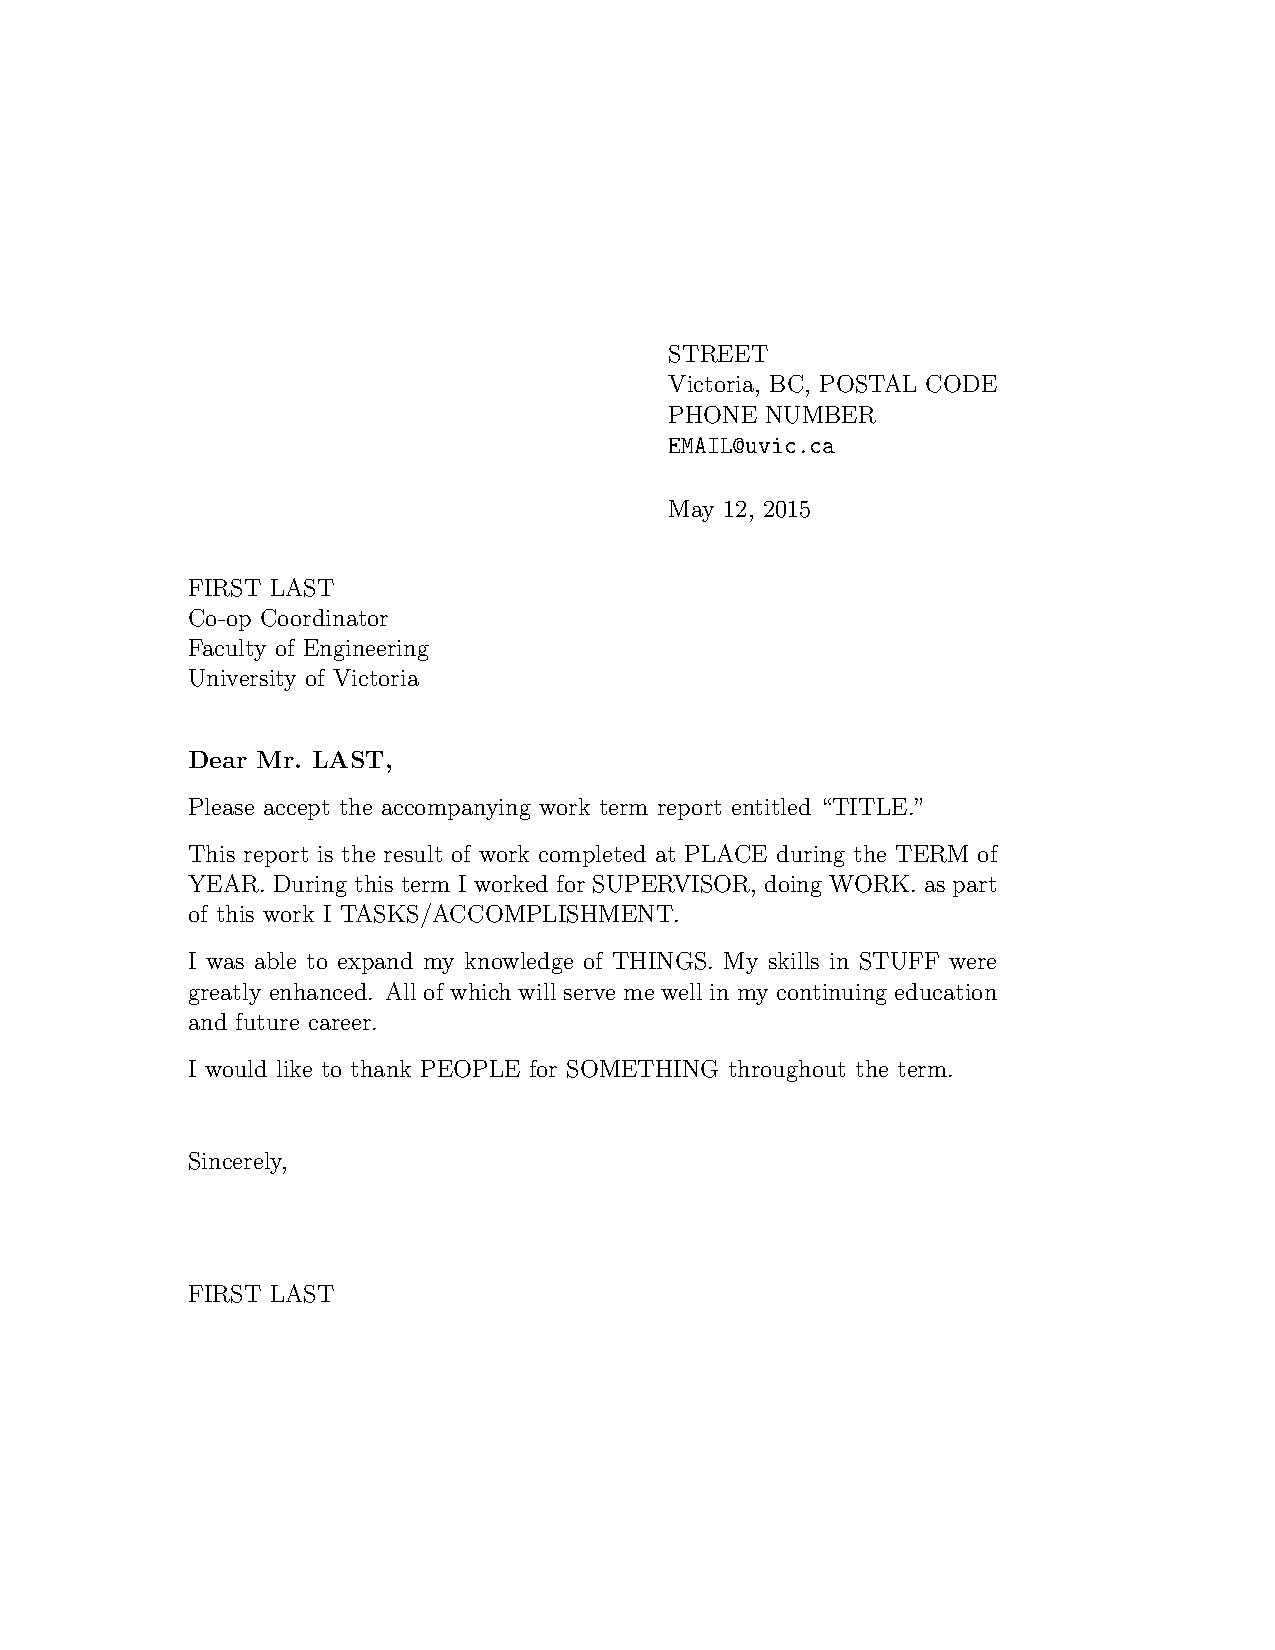
\includepdf[]{./Letter/letter.pdf} 


\newpage
%%%%%%%%%%%%%%%%%%%%%%%
%  Tables of Contents
%%%%%%%%%%%%%%%%%%%%%%%

\pagenumbering{roman}
%\setcounter{page}{1}
\tableofcontents


\phantomsection %fix hyperlinks
\vfill
\listoffigures \addcontentsline{toc}{section}{\listfigurename}

\vfill
\listoftables	\addcontentsline{toc}{section}{\listtablename}
\pagebreak


%%%%%%%%%%%%%%%%%%%%%%%
% 		Summary
%%%%%%%%%%%%%%%%%%%%%%%

\phantomsection %fix hyperlinks
\begin{Summary}
\doublespacing	
	
	Summary here
		
	
\end{Summary}


\pagebreak


%%%%%%%%%%%%%%%%%%%%%%%
% 		Glossary
%%%%%%%%%%%%%%%%%%%%%%%
\phantomsection %fix hyperlinks
\begin{Glossary}
	\item[Uvic] University of Victoria
\end{Glossary}


\newpage


%%%%%%%%%%%%%%%%%%%%%%%%%%%%%%%%%%%%%%%%%%%%%%%
%%%%          Document Starts Here      %%%%%%%

\doublespacing

\pagenumbering{arabic}
\section{Introduction}


Intro text



\section{Conclusions} \label{sec.conclusions}


\section{Recommendations} \label{sec.recommendations}

Recommendation text
	
\pagebreak

\singlespacing

%%%%%%%%%%%%%%%%%%%%%%%
% 	  Referrences
%%%%%%%%%%%%%%%%%%%%%%%
\pagebreak
\phantomsection %fix hyperlinks
\addcontentsline{toc}{section}{References}

\renewcommand*{\UrlFont}{\rmfamily} % prevent urls from font change
\printbibliography
references will go here, remove this line


%%%%%%%%%%%%%%%%%%%%%%%
% 	   Appendices
%%%%%%%%%%%%%%%%%%%%%%%

\begin{appendices}
	\addtocontents{toc}{\cftpagenumbersoff{section}} %removes appendix page numbers from toc


\Appendix{First Appendix}

	
	


\Appendix{Second Appendix} 

	

	
	
	\pagebreak %required for correct final page number
\end{appendices}	
\end{document}